\begin{frame}<5>{Factor analysis}
  % https://tex.stackexchange.com/questions/44449
  \newcommand*\grayout{}
  \alt<4>{\renewcommand\grayout{black}}{\renewcommand{\grayout}{black!40}}
  \small
  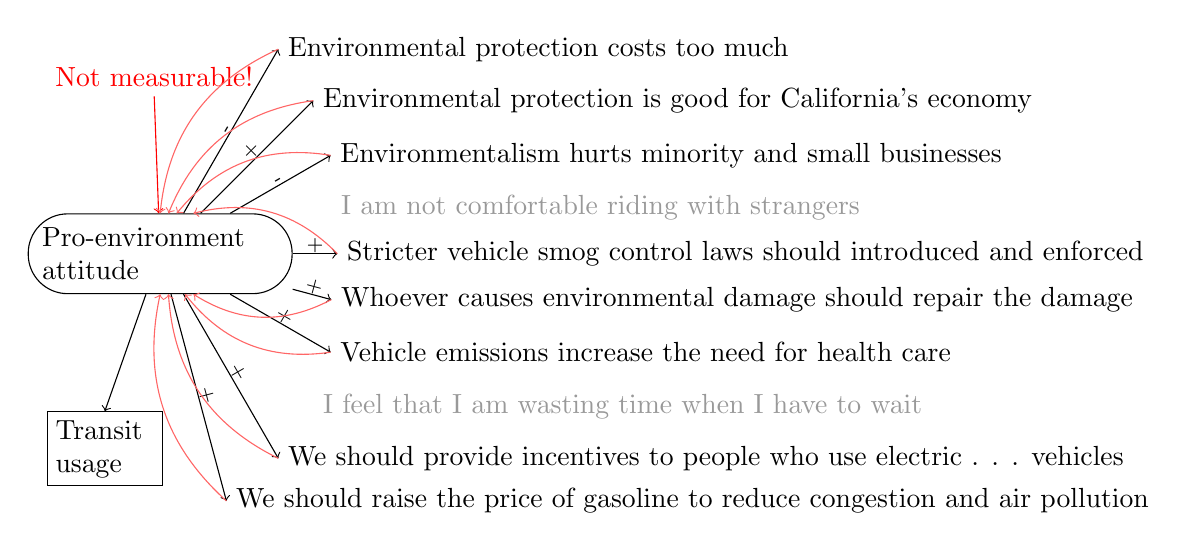
\begin{tikzpicture}
    \node[draw=black,inner sep=5pt,rounded corners=0.5cm,text width=3cm,anchor=east] (attitude) at (3, 5) {\normalsize  Pro-environment attitude};

    \draw[->] ([xshift=-2em]attitude) -- +(270:2cm) node[text=black,anchor=north,text width=1.25cm,inner sep=3pt,draw=black] { Transit usage };

    \pause

    \draw[<-,color=red] (attitude) -- +([xshift=-0.5ex] 90:2cm) node[text=red,anchor=south] {Not measurable!};

    \pause

    \node[anchor=west,text=black] (cost) at ([shift=({60:3cm})]attitude) {Environmental protection costs too much};
    \node[anchor=west,text=black] (econ) at ([shift=({45:2.75cm})]attitude) {Environmental protection is good for California’s economy};
    \node[anchor=west,text=black] (hurtssb) at ([shift=({30:2.5cm})]attitude) {Environmentalism hurts minority and small businesses};
    \node[anchor=west,text=\grayout] (strangers) at ([shift=({15:2.25cm})]attitude) {I am not comfortable riding with strangers};
    \node[anchor=west,text=black] (smog) at ([shift=({0:2.25cm})]attitude) {Stricter vehicle smog control laws should  introduced and enforced};
    \node[anchor=west,text=black] (damage) at ([shift=({345:2.25cm)})]attitude) {Whoever causes environmental damage should repair the damage};
    \node[anchor=west,text=black] (emissions) at ([shift=({330:2.5cm})]attitude) {Vehicle emissions increase the need for health care};
    \node[anchor=west,text=\grayout] (time) at ([shift=({315:2.75cm})]attitude) {I feel that I am wasting time when I have to wait};
    \node[anchor=west,text=black] (ev) at ([shift=({300:3cm})]attitude) {We should provide incentives to people who use electric . . . vehicles};
    \node[anchor=west,text=black] (raisegas) at ([shift=({285:3.25cm})]attitude) {We should raise the price of gasoline to reduce congestion and air pollution};
    \pause

    \draw[->] (attitude) -- (cost.west)
      node[yshift=-0.75ex, midway, above, sloped] {\scriptsize -};
    \draw[->] (attitude) -- (econ.west)
        node[yshift=-0.75ex, midway, above, sloped] {\scriptsize +};
    \draw[->] (attitude) -- (hurtssb.west)
        node[yshift=-0.75ex, midway, above, sloped] {\scriptsize -};
    \draw[->] (attitude) -- (smog.west)
        node[yshift=-0.75ex, midway, above, sloped] {\scriptsize +};
    \draw[->] (attitude) -- (damage.west)
        node[yshift=-0.75ex, midway, above, sloped] {\scriptsize +};
    \draw[->] (attitude) -- (emissions.west)
        node[yshift=-0.75ex, midway, above, sloped] {\scriptsize +};
    \draw[->] (attitude) -- (ev.west)
        node[yshift=-0.75ex, midway, above, sloped] {\scriptsize +};
    \draw[->] (attitude) -- (raisegas.west)
        node[yshift=-0.75ex, midway, above, sloped] {\scriptsize +};

    \pause

    \path[->,color=red!60,bend right] (cost.west) edge ([xshift=0pt]attitude.north);
    \path[->,color=red!60,bend right] (econ.west) edge ([xshift=3pt]attitude.north);
    \path[->,color=red!60,bend right] (hurtssb.west) edge ([xshift=6pt]attitude.north);
    \path[->,color=red!60,bend right] (smog.west) edge ([xshift=12pt]attitude.north);
    \path[->,color=red!60,bend left] (damage.west) edge ([xshift=12pt]attitude.south);
    \path[->,color=red!60,bend left] (emissions.west) edge ([xshift=9pt]attitude.south);
    \path[->,color=red!60,bend left] (ev.west) edge ([xshift=3pt]attitude.south);
    \path[->,color=red!60,bend left] (raisegas.west) edge ([xshift=0pt]attitude.south);


  \end{tikzpicture}

  {\tiny Based on \textcite{kitamura_micro-analysis_1997}}
\end{frame}

\begin{frame}{Factor analysis: unrotated factors}
  \begin{center}
    \includegraphics[width=0.5\textwidth]{fig/factor_no_rotation.pdf}\\
  \end{center}
  {\tiny Adapted from \textcite{kline_easy_1994} and \textcite{kitamura_micro-analysis_1997}; synthetic data.}
\end{frame}

\begin{frame}{Factor analysis: orthogonal rotation}
  \begin{center}
    \includegraphics[width=0.45\textwidth]{fig/factor_varimax.pdf}\\
  \end{center}
  {\tiny Adapted from \textcite{kline_easy_1994} and \textcite{kitamura_micro-analysis_1997}; synthetic data.}
\end{frame}

\begin{frame}{Factor analysis: oblique rotation, pattern matrix (regression coefficients)}
  \begin{center}
    \vspace*{-2cm}
    \includegraphics[width=0.65\textwidth]{fig/factor_oblimin_pattern.pdf}\\
  \end{center}
  \vspace*{-3cm}
  {\tiny Adapted from \textcite{kline_easy_1994} and\\\textcite{kitamura_micro-analysis_1997};\\synthetic data.}
\end{frame}

\begin{frame}{Factor analysis: oblique rotation, structure matrix (correlations)}
  \begin{center}
    \vspace*{-3cm}
    \includegraphics[width=0.55\textwidth]{fig/factor_oblimin_structure.pdf}\\
  \end{center}
  \vspace*{-3cm}
  {\tiny Adapted from \textcite{kline_easy_1994} and\\\textcite{kitamura_micro-analysis_1997};\\synthetic data.}
\end{frame}
